\documentclass[graphics]{beamer}

\usepackage{graphicx}
\usepackage{verbatim}
\usepackage{wrapfig}
\useoutertheme{shadow}
%\usecolortheme{orchid}
\usecolortheme{seahorse}


% math commands
\newcommand{\be}{\begin{eqnarray}}
\newcommand{\ee}{\end{eqnarray}}
\newcommand{\beq}{\begin{equation}}
\newcommand{\eeq}{\end{equation}}
\def\simless{\mathbin{\lower 3pt\hbox
      {$\rlap{\raise 5pt\hbox{$\char'074$}}\mathchar"7218$}}}
\def\simgreat{\mathbin{\lower 3pt\hbox
      {$\rlap{\raise 5pt\hbox{$\char'076$}}\mathchar"7218$}}} %> or of order

% variables

\def\toonscale{0.45}
\def\mboxy#1{\mbox{\small #1}}


\begin{comment}
\AtBeginSection[]{
  \frame{
    \frametitle{Outline}
    \tableofcontents[currentsection]
  }
}
\end{comment}

\title{Spin: Initial conditions
}
\subtitle{}
\author[U. Pen]{\textcolor{green}{Ue-Li Pen, ASIAA, CITA}
\\[8mm] 
}
\date{December 2, 2021}


\begin{document}

\frame{
\begin{picture}(320,250)
\put(-50,-130){
\includegraphics[width=5.5in]{Figures/delta_nu_sim.pdf}}
\end{picture}
\vspace{-3in}
\titlepage
}

%\section*{Introduction}
\section{Spin Alignments: probe of the early universe}

\begin{comment}
  \subsection{Outline}

  \frame{
    \frametitle{Outline}
    \tableofcontents
  }
\end{comment}

 
  \frame{
    \frametitle{Movie}
    {\tt http://cita.utoronto.ca/\~\,haoran/thnu/movie.html}
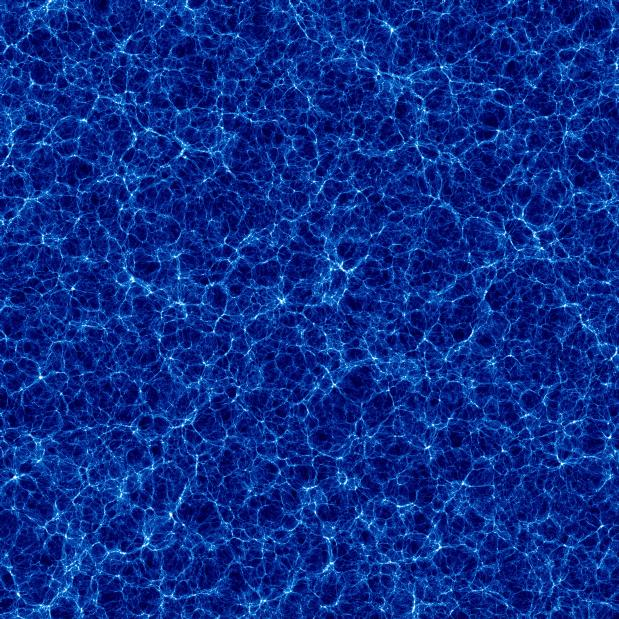
\includegraphics[width=4.2in]{Figures/thnucdmlowres.jpg}
}
  \frame{
    \frametitle{Galaxy Spins}
    \begin{itemize}
        \item most galaxies are rotating disks of stars and gas
        \item dust lanes, trailing spiral arms, HI velocity (rotation) field
        \item readily identifyable spin axis in 3-D (see Motloch talk)
        \item spin direction well preserved from initial conditions (Haoran's talk)
        \item potentially vast reservoir of fossils from initial conditions ($\gtrsim 10^8$ modes)
        \item direct probe of primordial helicity, cosmic neutrino background
     \end{itemize}
}
\frame{
    \frametitle{Observable}
\includegraphics[width=4.1in]{Figures/M51s.jpg}  

(M51, from Wikipedia)
  }

  \frame{
    \frametitle{Angular momentum (``spin'')}
    \begin{itemize}
        \item 1st order effect from misalignment of moment of inertia
          and tidal tensor
        \item torque: $\tau\equiv\int \rho \bf{r} \times \nabla \phi$
        \item Taylor expand: $\tau_i=\epsilon_{ijk} \int \rho x^jx^l \partial_l\partial_k\phi \equiv\epsilon_{ijk} I_{il}T_{lk}$
        \item Tensor form $\tau= * I \cdot T$
        \item first realized by S. White (1984), see also LP00
     \end{itemize}
}

  \frame{
%\vspace{-0.5in}
    \frametitle{predicting spin}
    \begin{itemize}
    \item Tidal Torque Theory (TTT): relates spin to initial Inertia and Tide
    \item Inertia tensor not easily identified, requires running N-body simulation.
    \item approximate Inertia by Tide (Zeldovich), torqued by external tide.
    \item IC-TTT: $j_\alpha=\epsilon_{\alpha\beta\gamma} {\cal T}_{\beta \kappa} {\cal T}^+_{\kappa\gamma}$
    \item ${\cal T}=\bar{\phi}_{,\beta\kappa}$ smoothed tidal field
    \item ${\cal T}^+_{\beta,kappa}=\bar{\phi}^+_{,\beta\kappa}$ tidal field smoothed on slightly larger scale, Taylor approximated by ${\cal T}^+_{\beta,kappa}=\bar{\rho}_{\beta\kappa}$
    \item $\sim$ 0.5 correlation with actual eulerian spin at optimal mass filter
    \item ``best one can hope for'' in data reconstruction
%          \vspace{-0.15in}
    \end{itemize}
    }
      

  \frame{
    \frametitle{E-mode Coordinate}
      reduce 3-D Lagrangian map to 1-D potential ({\it max Zeldovich}):
    \begin{eqnarray}      
{\rm potential\ deformation\ \ \ \ \ }  x^i &=& \xi^\mu \delta^i_\mu + \frac{\partial \phi}{\partial
    \xi^\mu}\delta^{i\mu}\nonumber\\
{\rm dreibein\ \ \ \ \ \  } e^i_\mu &\equiv& \partial x^i / \partial \xi ^ \mu \nonumber\\
 {\rm volume\  element\ \ \ \ }\sqrt{g} &\equiv& \mathrm{det}\left| e^i_\mu\right|\nonumber\\
{\rm mass\ coordinate \ \ \ \ \ }    \rho \sqrt{g}&=&\mathrm{Const.}\nonumber\\
    \partial _\mu (\rho \sqrt{g} e^\mu _i \delta^{i\nu}
    \partial_\nu \dot{\phi})&=&\langle\rho\rangle-\rho \sqrt{g}
\label{eqn:dif}
\end{eqnarray}
Solve Monge-Amp\'ere eqn (\ref{eqn:dif}) using multigrid (Pen 1995):
unique bijective mass coordinate.  See also Tully/Peebles, Mohayaee+, Goldberg, Schmidtfull, Wang+, Seljak,
Zaldarriaga, Hada/Eisenstein, Shi/Brikin/Li+, Jasche+, Sarpa+
}

\frame{
    \frametitle{3-D: E-mode Lagrangian}
%\vspace{-0.5in}
\hspace{-0.2in}\includegraphics[width=2.1in]{Figures/nonlinear.png}  
\vspace{0.15in}\includegraphics[width=2.1in]{Figures/reconstructed.png}  

Eulerian (L) vs Lagrangian (R) (from Yu et al 2016, 1610.7112)
  }

\frame{
    \frametitle{Lagrangian coordinates}
\center{\includegraphics[width=4.3in]{Figures/delta_reco_raw.pdf}  }
  }

  \frame{
    \frametitle{Multigrid solution}
\vspace{-0.7in}\center{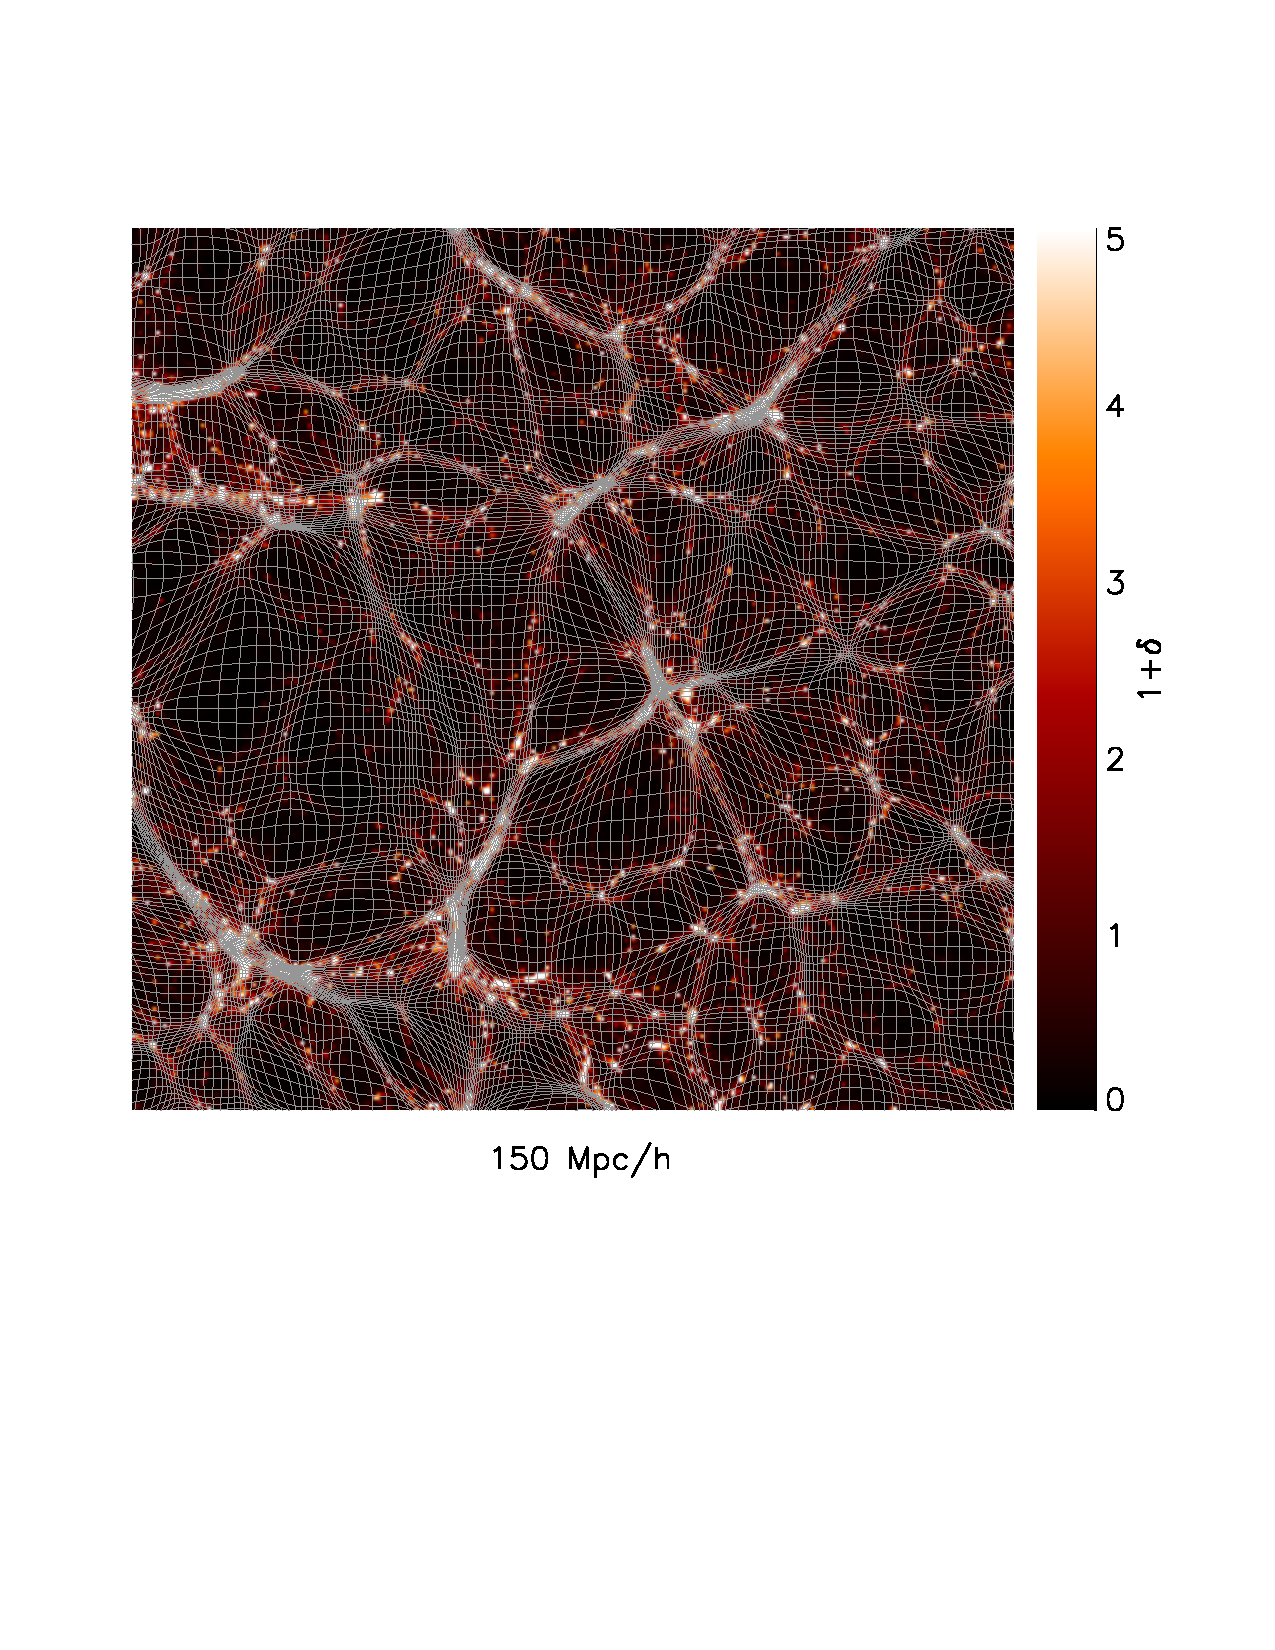
\includegraphics[width=4.0in]{Figures/map0512-0128_i1500_xz222.pdf}}
Zhu et al 1610.09638
}
  \frame{
    \frametitle{Redshift space}
Zhu et al 1610.09638
\vspace{-0.7in}\center{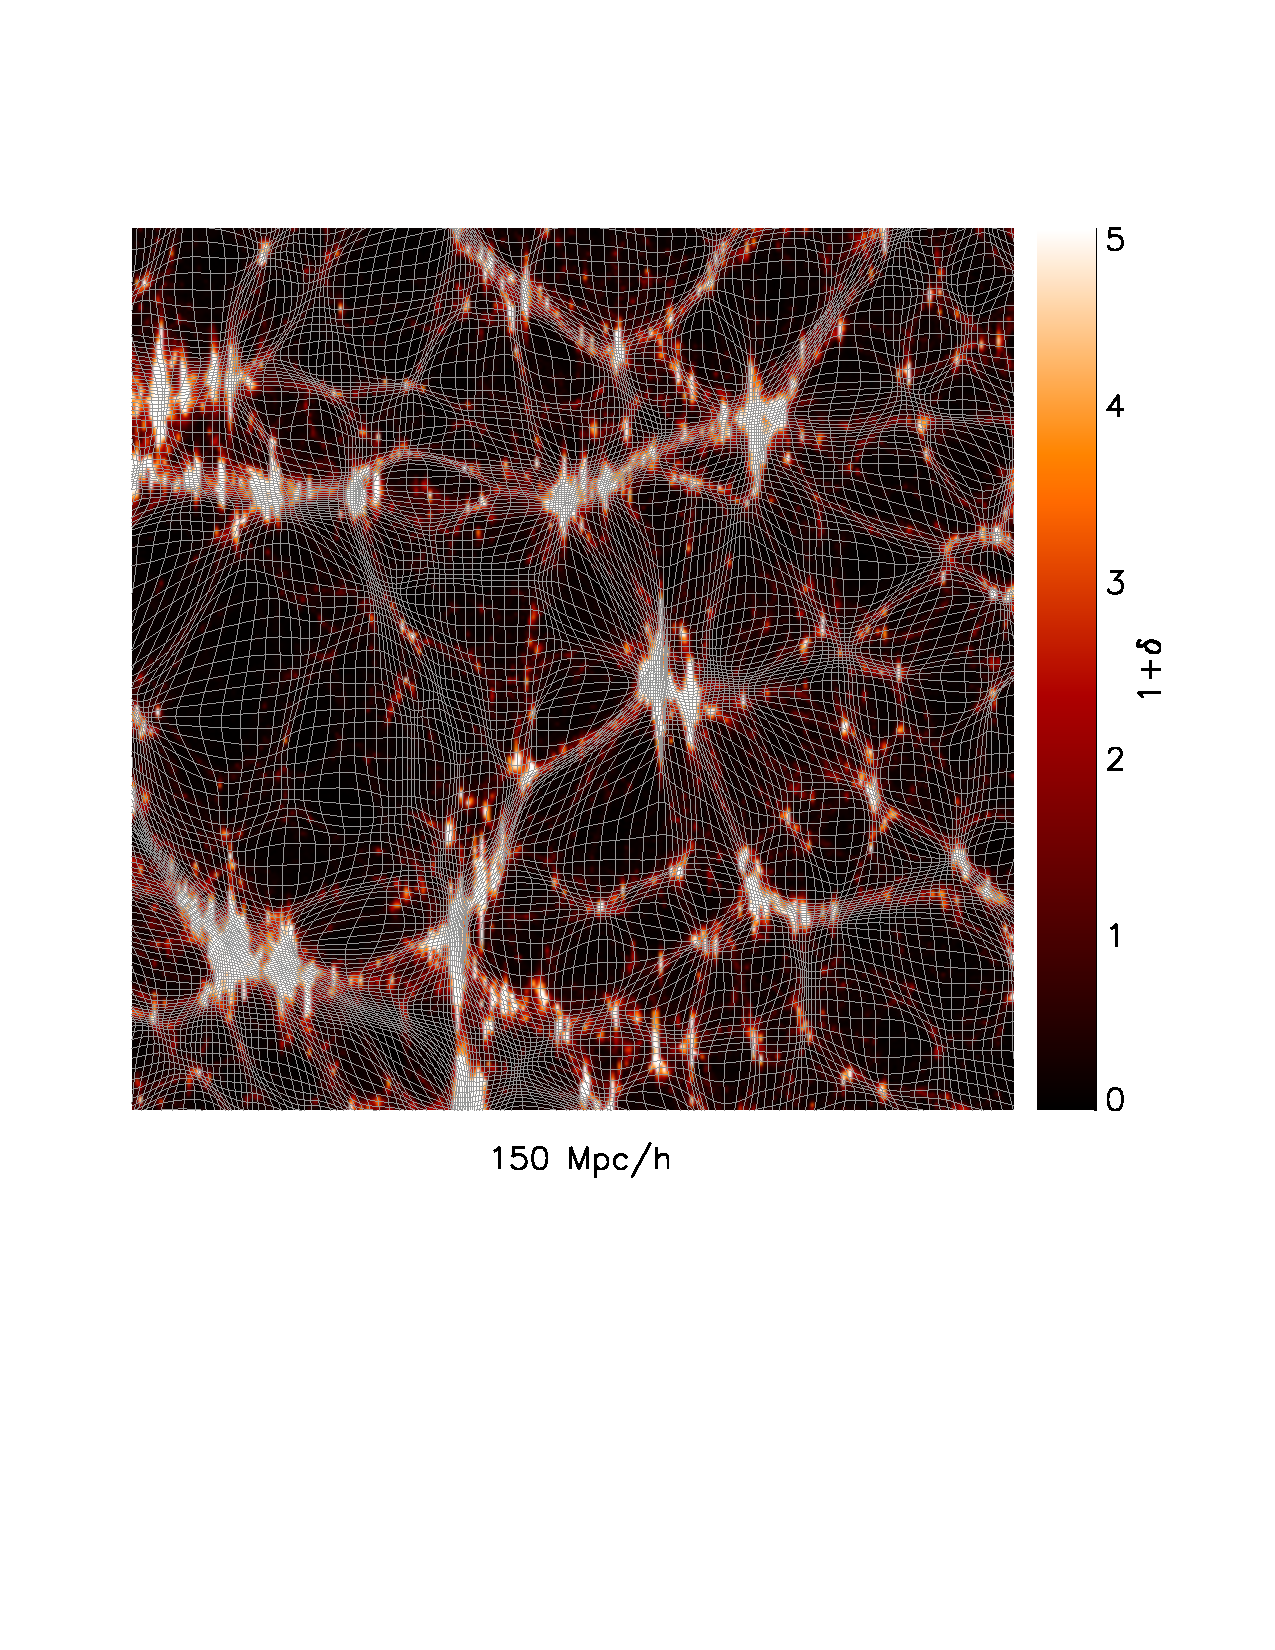
\includegraphics[width=4.0in]{Figures/map0512-0128_i0900_xz222_rsd3.pdf}}
}

  \frame{
    \frametitle{Low noise limit}
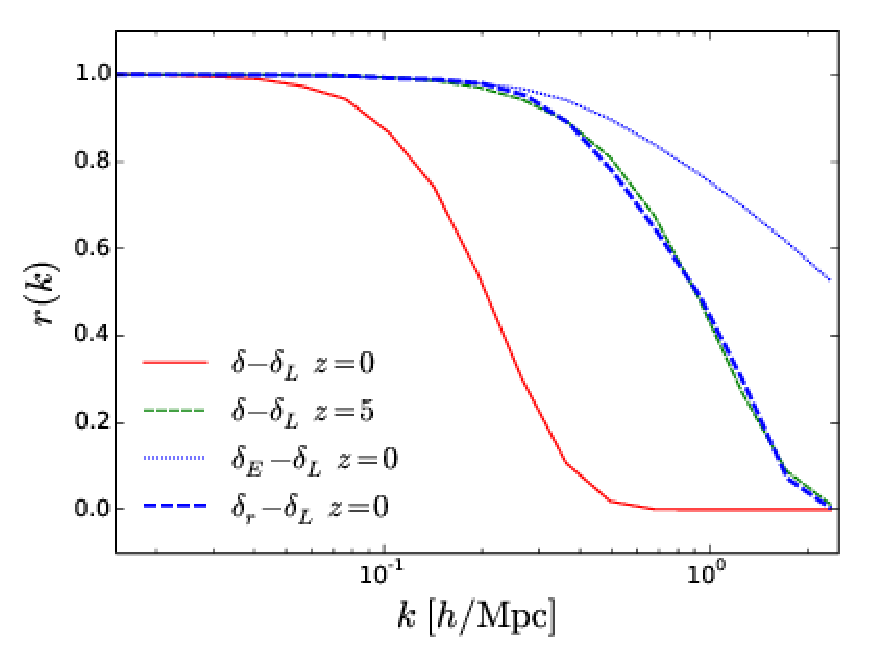
\includegraphics[width=3.4in]{Figures/rk.pdf}
}
  \frame{
    \frametitle{Halos}
\vspace{-0.5in}\hspace{-0.9in}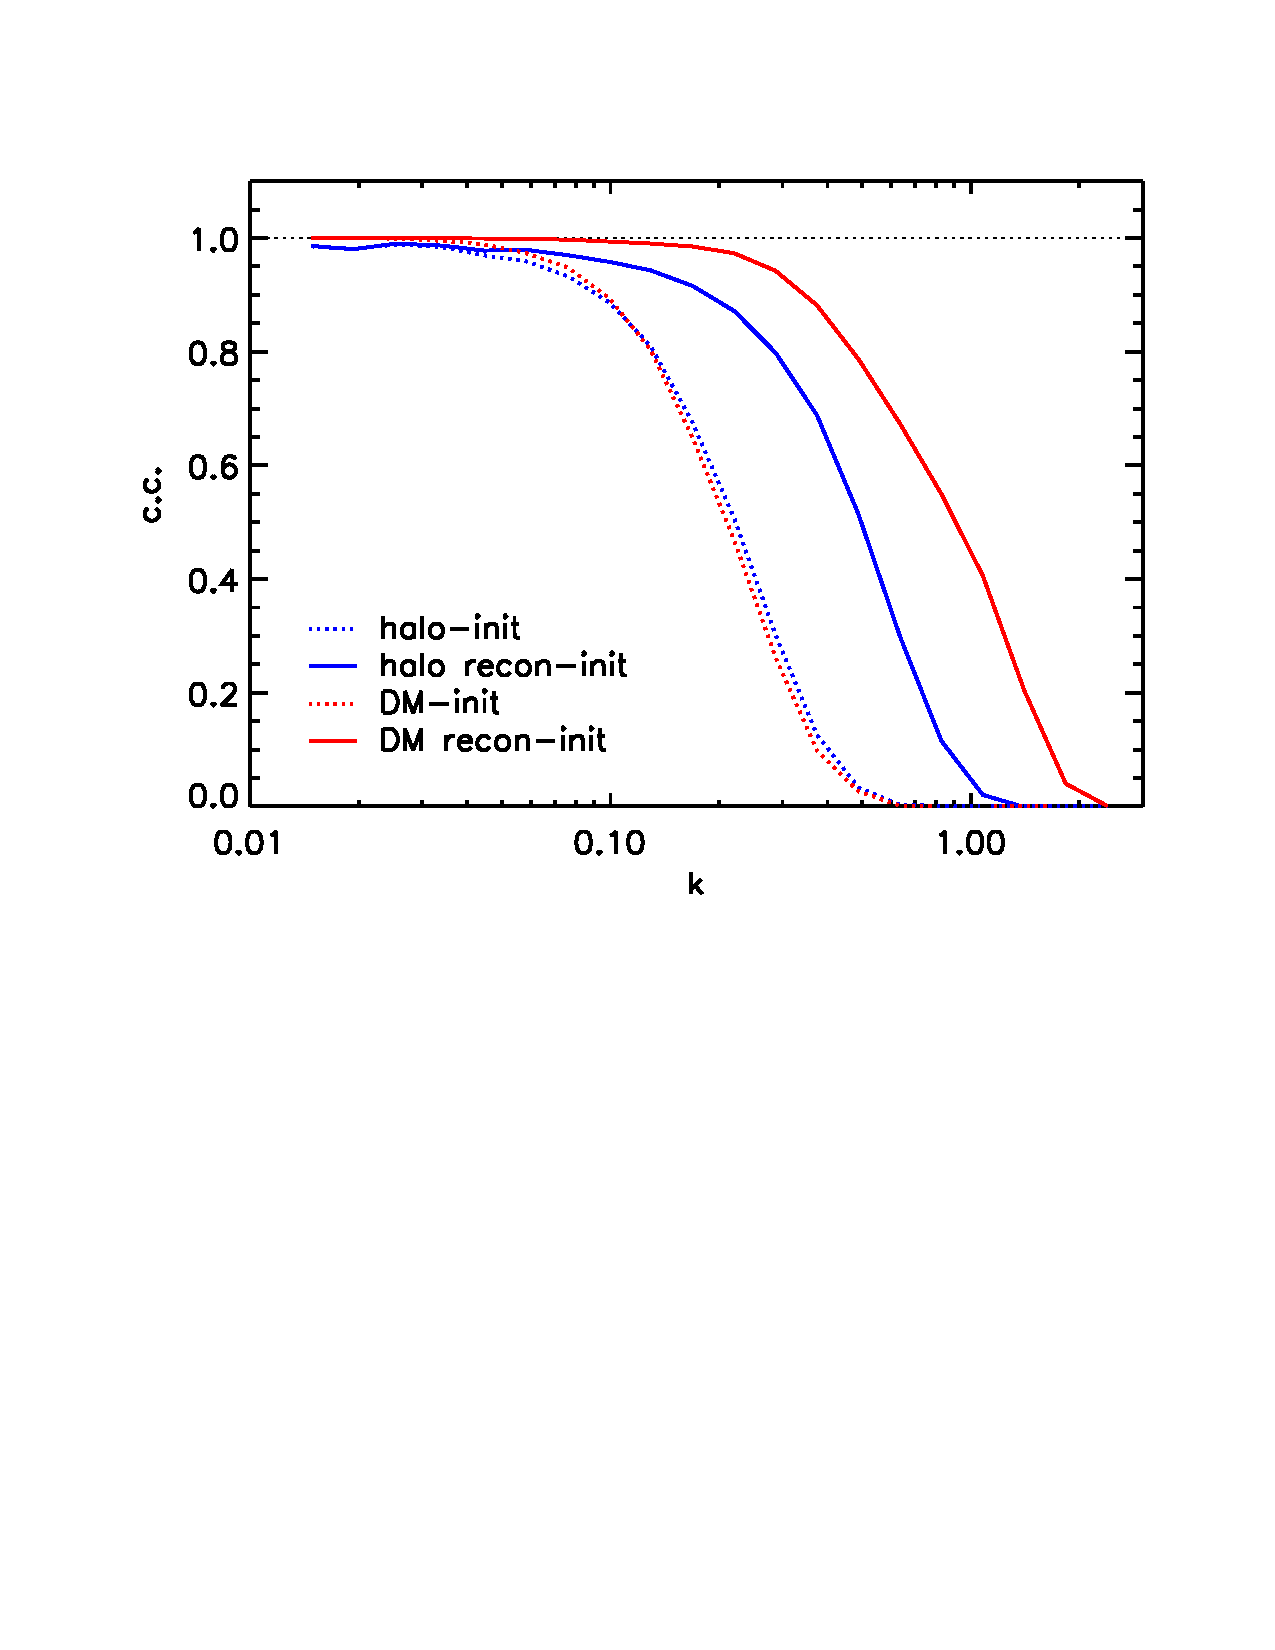
\includegraphics[width=5.0in]{Figures/halocc.pdf}
}

 \frame{
    \frametitle{Predicting Neutrino Torques}
    \begin{itemize}
      \item $\nu$ gravitational field (large scale tide) torques CDM (small scale inertia)
      \item $\Delta x (q) = q^j \partial_i\partial_j \psi$
        \item $I_c \sim T_c$: both describe particle displacement
        \item $j_\nu = \epsilon T_c T_\nu$
        \item Neutrino tidal torque is predictable observable from
          displacement potential
     \end{itemize}
  }
  \frame{
    \frametitle{Illustration}
\vspace{-0.5in}\hspace{-0.6in}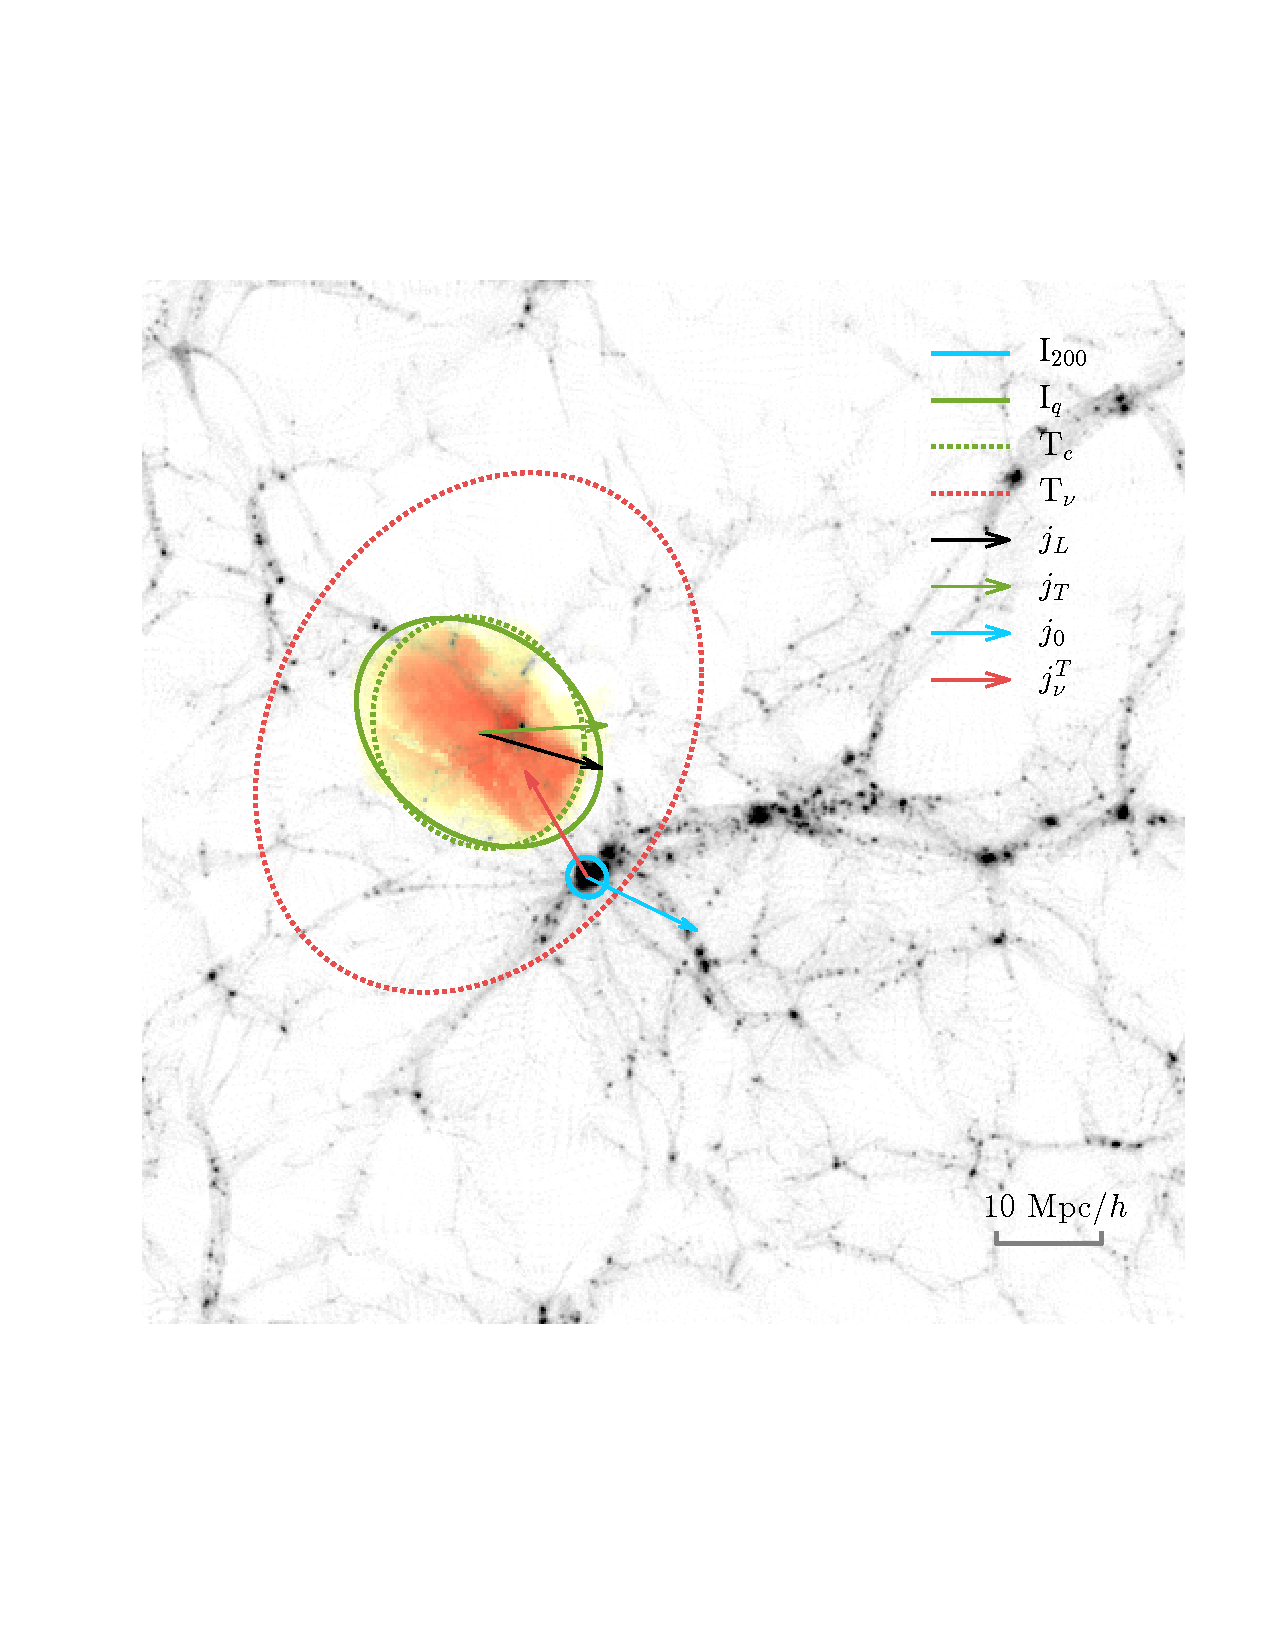
\includegraphics[width=5.0in]{Figures/f1.pdf}
}

 \frame{
    \frametitle{Size estimate}
    \begin{itemize}
    \item $|j_\nu/j_c| \sim 10^{-4} (f_\nu /0.003) [\sqrt{P(k_{\rm FS})/P(k_{\rm vir})}/0.03]$
    \item agrees with simulation measurement
    \item need $n> 10^8$ galaxy spins
    \item accessible in next generation 21cm surveys
     \end{itemize}
  }


  \frame{
\vspace{-0.5in}
    \frametitle{Future 21cm Surveys}
    \begin{itemize}
        \item expand on HSHS (Peterson et al 2006), CHIME
        \item build on economy of scale, map $10^{11}$ galaxies
     \end{itemize}
  }
  
\frame{
\vspace{-0.5in}
    \frametitle{More cosmological applications}
    \begin{itemize}
        \item map initial (linear) tidal field
        \item BAO, standard ruler (Alcock-Paczynski effect)
        \item modified gravity, time evolving neutrino mass
     \end{itemize}
  }


\frame{
\vspace{-0.5in}
    \frametitle{Conclusions}
    \begin{itemize}
      \item galaxy spins: new probe of initial conditions
      \item predictable from observable displacement field using
        non-linear reconstruction
      \item computationally straightforward, mass coordinate
            similar to Lagrangian
          \item already observable, scalable to much larger surveys
          \item parity odd field, less likely to be contaminated
          \item enables measurement of 2 cosmic scalar fields:
            potential beat cosmic variance limits, etc
     \end{itemize}
  }


\end{document}
